\documentclass{article}

\usepackage{amsmath}
\usepackage{amsfonts}
\usepackage{amssymb}
\usepackage[utf8]{inputenc}
\usepackage{graphicx}
\usepackage{subcaption}
\usepackage[margin=0.5in]{geometry}

\title{Taller 3}
\author{Miguel A. Gomez B.}

\begin{document}
	\maketitle
\paragraph{}\textit{(25 points)} Write a python function \textbf{FourierSeries(f,P,x,n)} that return the values of the Fourier series of the function $f(x)$ at the point $x$. Plot the Fourier series of the following functions:
$$f(x) = 1-x$$
$$f(x) = x^2,$$
using $P=1$, but calculate the series on the interval $(-2P, 2P)$. Repeat the plot for $n = 6, 12, 36, 124$. What do you observe as $n$ becomes larger?

\paragraph{} For $f(x) = 1-x$
\begin{figure}[h!]
	\centering
	\begin{subfigure}[b]{0.2\linewidth}
		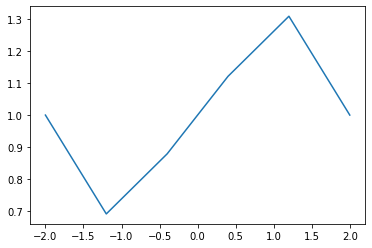
\includegraphics[width=\linewidth]{img/f1_n6.png}
		\caption{n=6}
	\end{subfigure}
	\begin{subfigure}[b]{0.2\linewidth}
		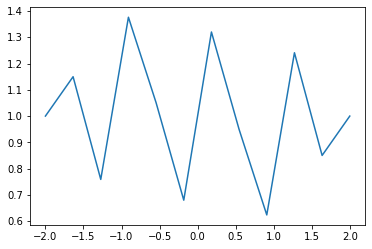
\includegraphics[width=\linewidth]{img/f1_n12.png}
		\caption{n=12}
	\end{subfigure}
	\begin{subfigure}[b]{0.2\linewidth}
		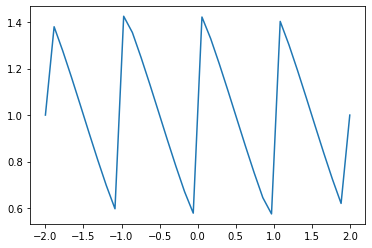
\includegraphics[width=\linewidth]{img/f1_n36.png}
		\caption{n=36}
	\end{subfigure}
	\begin{subfigure}[b]{0.2\linewidth}
		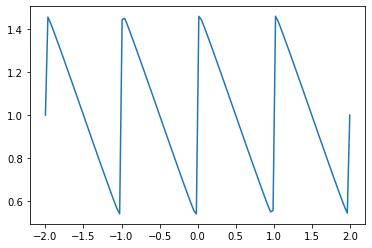
\includegraphics[width=\linewidth]{img/f1_n124.png}
		\caption{n=124}
	\end{subfigure}
\end{figure}
\paragraph{} For $f(x) = x^2$
\begin{figure}[h!]
	\centering
	\begin{subfigure}[b]{0.2\linewidth}
		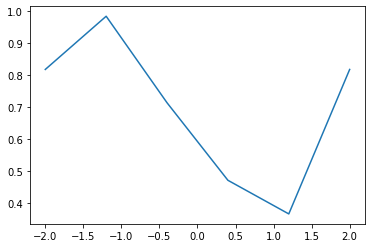
\includegraphics[width=\linewidth]{img/f2_n6.png}
		\caption{n=6}
	\end{subfigure}
	\begin{subfigure}[b]{0.2\linewidth}
		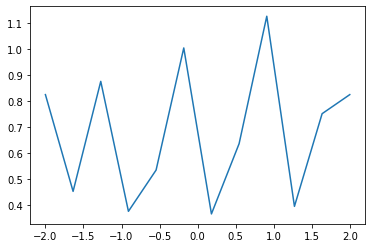
\includegraphics[width=\linewidth]{img/f2_n12.png}
		\caption{n=12}
	\end{subfigure}
	\begin{subfigure}[b]{0.2\linewidth}
		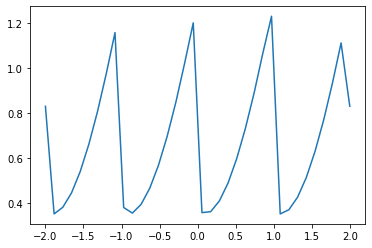
\includegraphics[width=\linewidth]{img/f2_n36.png}
		\caption{n=36}
	\end{subfigure}
	\begin{subfigure}[b]{0.2\linewidth}
		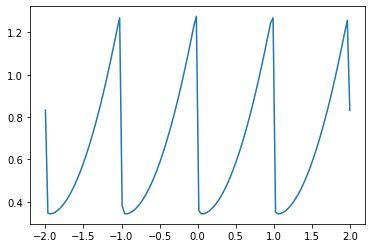
\includegraphics[width=\linewidth]{img/f2_n124.png}
		\caption{n=124}
	\end{subfigure}
\end{figure}
\begin{center}
	The code file to built this figures is named \textit{RunMeInPython.py}.
\end{center}
\paragraph{} As n increases, the Fourier series oscillate in shorter periods, which is similar to the behavior of the trigonometric functions (that compose the series), also, if we increase the number of points on the same interval we see that at some level the same behavior arises:
\begin{center}
\begin{figure}[h!]
	\centering
	\begin{subfigure}[b]{0.2\linewidth}
		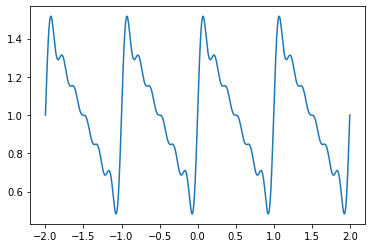
\includegraphics[width=\linewidth]{img/f1_n6_more.png}
		\caption{n=6 for $f(x) = 1-x$}
	\end{subfigure}
	\begin{subfigure}[b]{0.2\linewidth}
		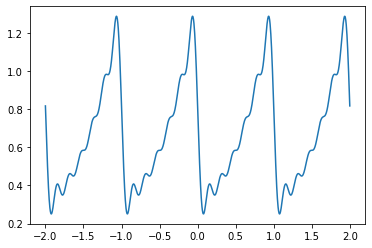
\includegraphics[width=\linewidth]{img/f2_n6_more.png}
		\caption{n=6 for $f(x) = x^2$}
	\end{subfigure}
\end{figure}
\end{center}
but I'm not sure why exactly this occurs.
\paragraph{}\textit{(10 Points)} Test the stability of the zero solution for the following system.
$$x_1' = -4x_1 + 8x_1x^2_2$$
$$x_2' = -12x^2_1x_2 - 6x^2$$

\end{document}